%
% 6.006 problem set 4 solutions template
%
\documentclass[tikz, 12pt,twoside]{article}

\usepackage{amsmath}
\usepackage{color}
\usepackage{algorithm}
\usepackage{marvosym}
\usepackage[noend]{algpseudocode}

\usepackage{graphicx}
\usepackage{placeins}
\usepackage{hyperref}

\usepackage{tikz}
\usetikzlibrary{angles, arrows.meta, quotes}
\usepackage{siunitx}

\setlength{\oddsidemargin}{0pt}
\setlength{\evensidemargin}{0pt}
\setlength{\textwidth}{6.5in}
\setlength{\topmargin}{0in}
\setlength{\textheight}{8.5in}

\newcommand{\theproblemsetnum}{1}
\newcommand{\releasedate}{September 13, 2016}

\newcommand{\tabUnit}{3ex}
\newcommand{\tabT}{\hspace*{\tabUnit}}

\title{8.012 Problem Set 1}

\begin{document}
\delimitershortfall=-1pt

\centering
\textbf{8.012 Problem Set 1} \\
\href{https://ocw.mit.edu/courses/physics/8-012-physics-i-classical-mechanics-fall-2008/assignments/ps1.pdf}{Link}
\centering

\setlength{\parindent}{0pt}

\medskip

\hrulefill

%%%%%%%%%%%%%%%%%%%%%%%%%%%%%%%%%%%%%%%%%%%%%%%%%%%%%
% See below for common and useful latex constructs. %
%%%%%%%%%%%%%%%%%%%%%%%%%%%%%%%%%%%%%%%%%%%%%%%%%%%%%

% Some useful commands:
%$f(x) = \Theta(x)$
%$T(x, y) \leq \log(x) + 2^y + \binom{2n}{n}$
% {\tt code\_function}


% You can create unnumbered lists as follows:
%\begin{itemize}
%    \item First item in a list 
%        \begin{itemize}
%            \item First item in a list 
%                \begin{itemize}
%                    \item First item in a list 
%                    \item Second item in a list 
%                \end{itemize}
%            \item Second item in a list 
%        \end{itemize}
%    \item Second item in a list 
%\end{itemize}

% You can create numbered lists as follows:
%\begin{enumerate}
%    \item First item in a list 
%    \item Second item in a list 
%    \item Third item in a list
%\end{enumerate}

% You can write aligned equations as follows:
%\begin{align} 
%    \begin{split}
%        (x+y)^3 &= (x+y)^2(x+y) \\
%                &= (x^2+2xy+y^2)(x+y) \\
%                &= (x^3+2x^2y+xy^2) + (x^2y+2xy^2+y^3) \\
%                &= x^3+3x^2y+3xy^2+y^3
%    \end{split}                                 
%\end{align}

% You can create grids/matrices as follows:
%\begin{align}
%    A = 
%    \begin{bmatrix}
%        A_{11} & A_{21} \\
%        A_{21} & A_{22}
%    \end{bmatrix}
%\end{align}

\begin{itemize}
\item \textbf{1.} \emph{Kleppner \& Kolenkow, Problem 1.2} \\ \vspace{5mm}
  Let $\mathbf{A} = (3\mathbf{\hat{i}} - 2\mathbf{\hat{j}} + 5\mathbf{\hat{k}})$ and $\mathbf{B} = (6\mathbf{\hat{i}} - 7\mathbf{\hat{j}} + 4\mathbf{\hat{k}})$.
  \begin{itemize}
  \item \textbf{(a)}
    $\mathbf{A}^{2} = \mathbf{A} \cdot \mathbf{A} = 3^{2} + (-2)^{2} + 5^{2} = 9 + 4 + 25 = \mathbf{38}$
  \item \textbf{(b)}
    $\mathbf{B}^{2} = \mathbf{B} \cdot \mathbf{B} = 6^{2} + (-7)^{2} + 4^{2} = 36 + 49 + 16 = \mathbf{101}$
  \item \textbf{(c)}
    $(\mathbf{A}\cdot\mathbf{B})^{2} = \left((3*6) + (-2*-7) + (5*4)\right)^{2} = (18 + 14 + 20)^{2} = 52^{2} = \mathbf{2704}$
  \end{itemize}

\item \textbf{2.} \emph{Kleppner \& Kolenkow, Problem 1.7} \\ \vspace{5mm}

  Let $\mathbf{A}$, $\mathbf{B}$, $\mathbf{C}$ define a triangle, as below.
  \begin{figure}[H]
    \centering
      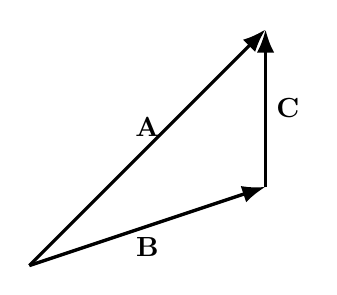
\begin{tikzpicture}[
    > = Straight Barb,
    vector/.style = {very thick,-{Latex}},
    angles/.style = {draw, <->, angle eccentricity=1,
      right, angle radius=7mm}
    ]
    \draw[vector] (0,0) -- (3,3) node[midway, left, above] {$\mathbf{A}$};
    \draw[vector] (0,0) -- (3,1) node[midway, below] {$\mathbf{B}$};
    \draw[vector] (3,1) -- (3,3) node[midway, right] {$\mathbf{C}$};
    \end{tikzpicture}
  \end{figure}

  We have that

  \begin{align*}
    \mathbf{A} &= \mathbf{B} + \mathbf{C} \\
    \mathbf{B} &= \mathbf{A} - \mathbf{C} \\
    \mathbf{C} &= \mathbf{A} - \mathbf{B} \\
  \end{align*}

  then

  \begin{align*}
    \left|\mathbf{A}\times\mathbf{B}\right| &= \mathit{A}\mathit{B}\sin{\theta_{\mathbf{A}\mathbf{B}}}
    = |(\mathbf{B} + \mathbf{C}) \times \mathbf{B}| = |\mathbf{C} \times \mathbf{B}| \\
    \left|\mathbf{C}\times\mathbf{B}\right| &= \mathit{C}\mathit{B}\sin{\theta_{\mathbf{C}\mathbf{B}}}
    = |\mathbf{C} \times (\mathbf{A} - \mathbf{C})| = |\mathbf{C} \times \mathbf{A}| \\
    \left|\mathbf{C}\times\mathbf{A}\right| &= \mathit{C}\mathit{A}\sin{\theta_{\mathbf{C}\mathbf{A}}} \\
  \end{align*}

  Thus,

  $$
  \mathit{A}\mathit{B}\sin{\theta_{\mathbf{A}\mathbf{B}}} = \mathit{C}\mathit{B}\sin{\theta_{\mathbf{C}\mathbf{B}}} = \mathit{C}\mathit{A}\sin{\theta_{\mathbf{C}\mathbf{A}}}
  $$

  Dividing by $ABC$, we see:

  $$
  \frac{\sin{\theta_{\mathbf{A}\mathbf{B}}}}{C} = \frac{\sin{\theta_{\mathbf{C}\mathbf{B}}}}{A} = \frac{\sin{\theta_{\mathbf{C}\mathbf{A}}}}{B}
  $$
  as desired.



\item \textbf{3.} \emph{Kleppner \& Kolenkow, Problem 1.12} \\ \vspace{5mm}
  Let $\mathbf{r}_1$ and $\mathbf{r}_2$ be two points separated by distance $r = |\mathbf{r}_1 - \mathbf{r}_2|$. Then $\mathbf{r}_2 - \mathbf{r}_1$
  points in the direction from $\mathbf{r}_1$ to $\mathbf{r}_2$. If $x$ is any number, then $(\mathbf{r}_2 - \mathbf{r}_1)x$ points in the same
  (or opposite) direction, but has magnitude $xr$ (recall that $(\mathbf{r}_2 - \mathbf{r}_1)$ has magnitude $r$ by definition). Then
  $\mathbf{A} = \mathbf{r}_1 + (\mathbf{r}_2 - \mathbf{r}_1)x$ points from the origin to a point on the line between $\mathbf{r}_1$
  and $\mathbf{r}_2$ at a distance $x$ from $\mathbf{r}_1$.

\item \textbf{4.} \emph{Kleppner \& Kolenkow, Problem 1.13} \\ \vspace{5mm}

\item \textbf{9.} \\ \vspace{5mm}
  \begin{itemize}
  \item \textbf{(a)}
  \item \textbf{(b)}
    Observe that the both trains travel at speed $v$ over a distance $d/2$, and meet after a time $d/(2v)$.
    The bee thus gets crushed at time $d/(2v)$, and travels at speed $u$ until then. It's obvious then that
    the bee travels a distance of $ud/(2v)$ in total.
  \end{itemize}
\end{itemize}

\end{document}

